%%%%%%%%%%%%%%%%%%%%%%%%%%%%%%%%%%%%%%%%%%%%%%%%%%%%%%
%%%%%%%%%%%%%%%%%%%%%%%%%%%%%%%%%%%%%%%%%%%%%%%%%%%%%%
%%%%%%%%%%%%%%%%%%%%%%%%%%%%%%%%%%%%%%%%%%%%%%%%%%%%%%
\subsection{Standard Model like toys}

Standard Model like toys are signal free (no singal injection) in which we use
 $Z$~boson cross section give SM to generate toys. In this type of models toy data points
 only contain statistical uncertainty. Thus, toy data points are randomly 
 distributed around 1 according to statistical fluctuation.
In figure~\ref{fig:SM_like_toy_scrambled}, the error bar
 on each data point is statistical uncertainty. The left plot show one of
  the original toy dataset, and the right plot is it's corresponding scrambled version.
  The scrambled verions of SM like toys are also randomly distributed around 1 
  according to statistical fluctuation.
 

\begin{figure}[hp]
\centering
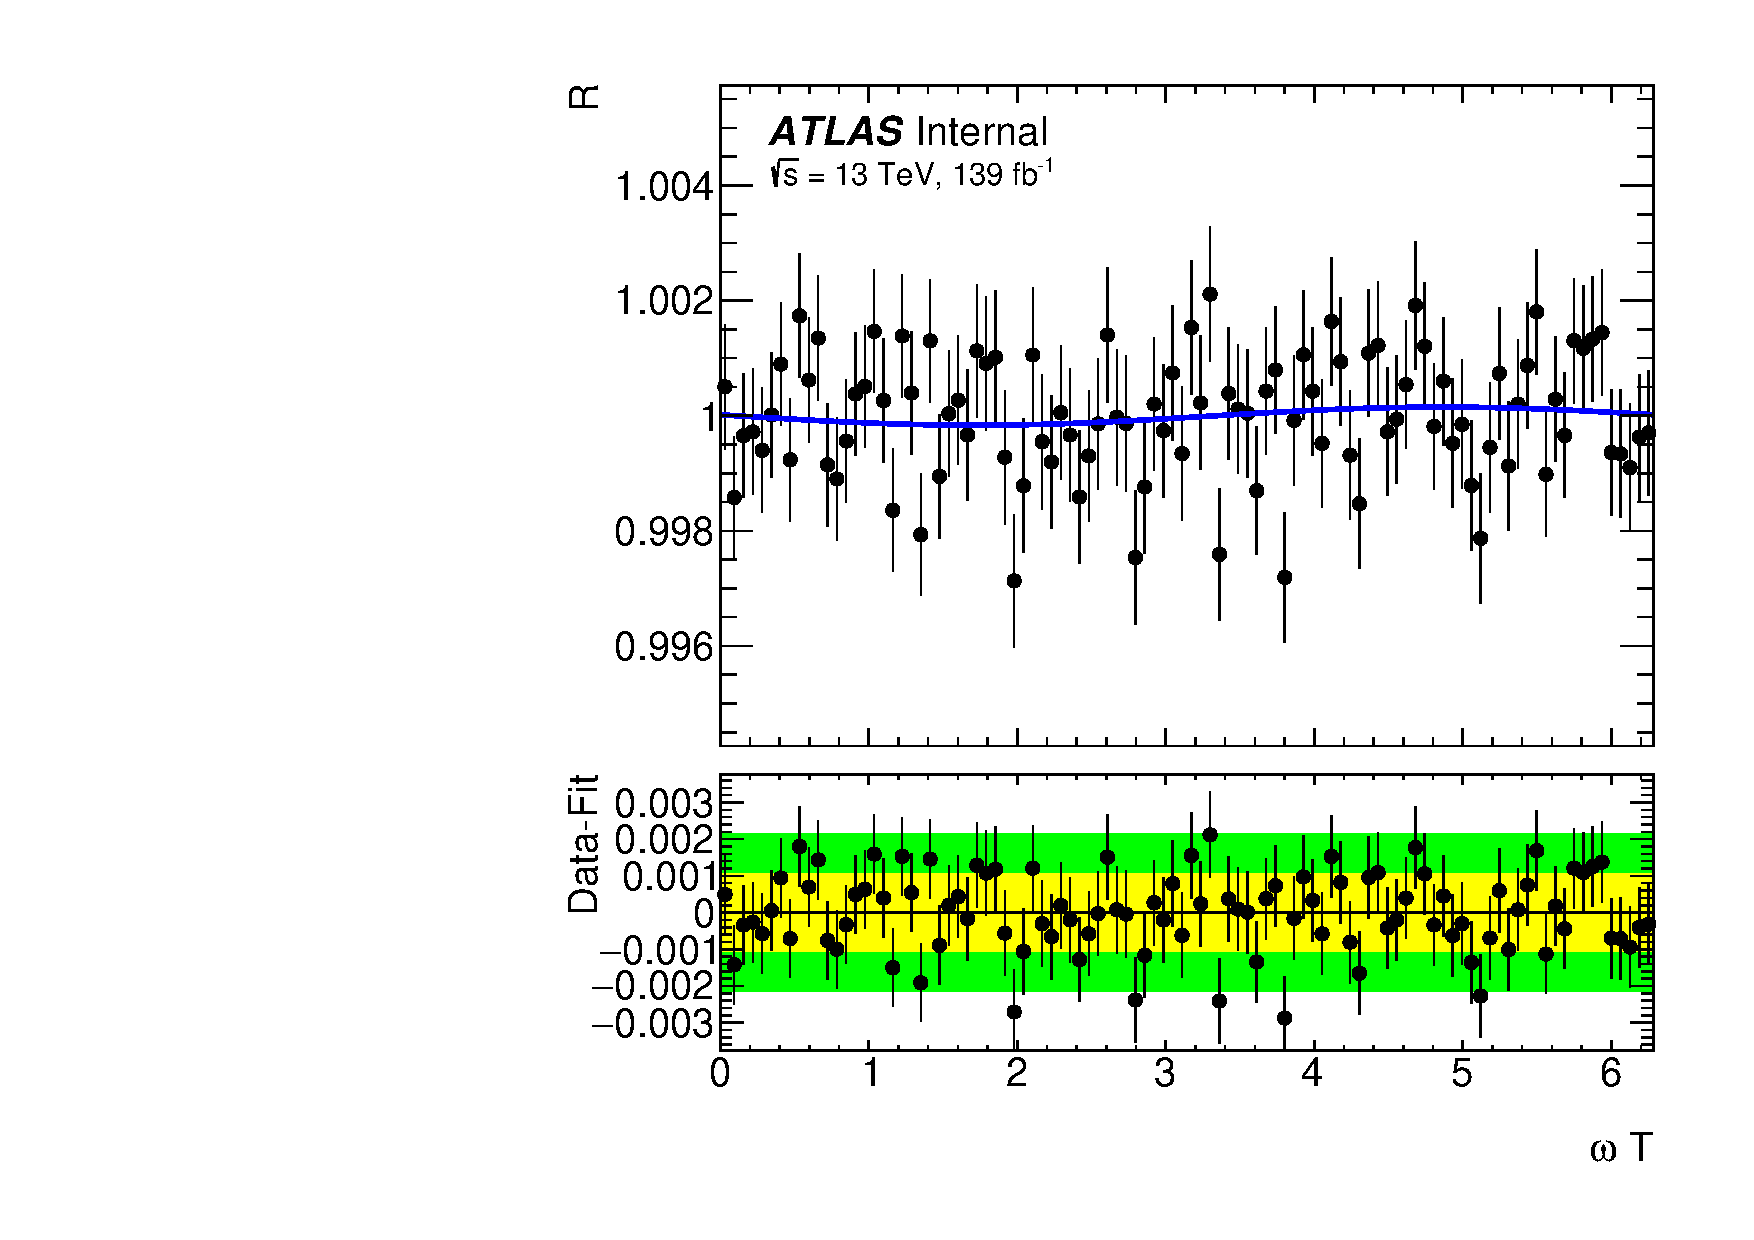
\includegraphics[width=0.45\textwidth]{figs/scrambling/fit_results_d[u,X,Z]_101_residual_12func_SM}
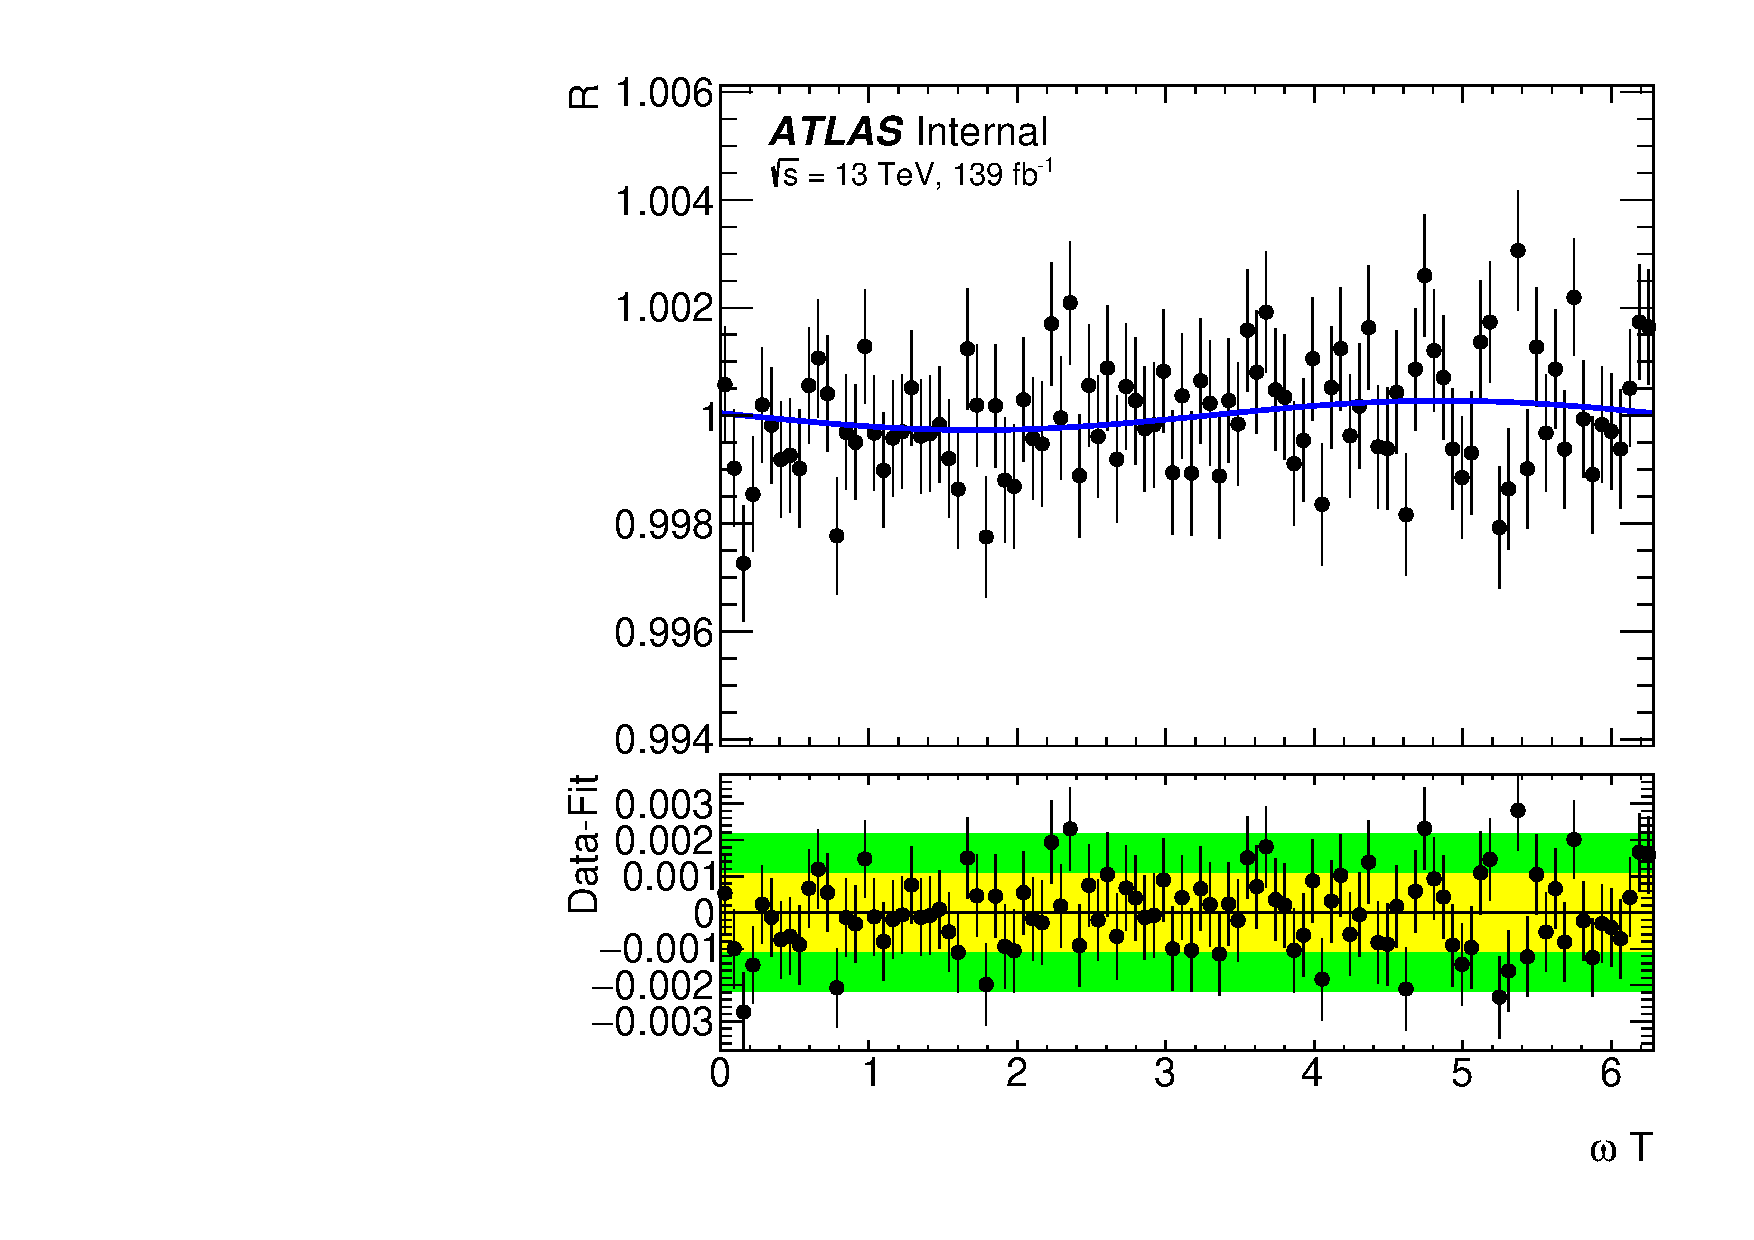
\includegraphics[width=0.45\textwidth]{figs/scrambling/fit_results_d[u,X,Z]_101_residual_12func_SM_scrampled}
\caption{SM-like toy dataset (left), which corresponds to full Run 2 luminosity, 
and scrambled SM-like toy dataset (right). SM-like toys are signal-free datsets
 ($\sigma_{LIV}/\sigma_{SM} = 0$). The X-axis is the sidereal phase, $\omega T$.
  The blue line corresponds to the $d_{u}^{X,Z}$ signal shape after fit to the 
  toy dataset. Bottom panel in each plot is the residual (data-fit)}
\label{fig:SM_like_toy_scrambled}
\end{figure}



Figure~\ref{fig:SM_like_toy_fit_results12} show fit results of SM like toys
 and their scrambled versions. The black points are average of 1000 fit results,
 and the green and yellow bands are corresponding one and two standard diviation.
 As we epected, the average fit results of MS like toys and their scrambled versions
  are in good agreement with each other and with zero since they
 are signal free toys.



\begin{figure}[hp]
\centering
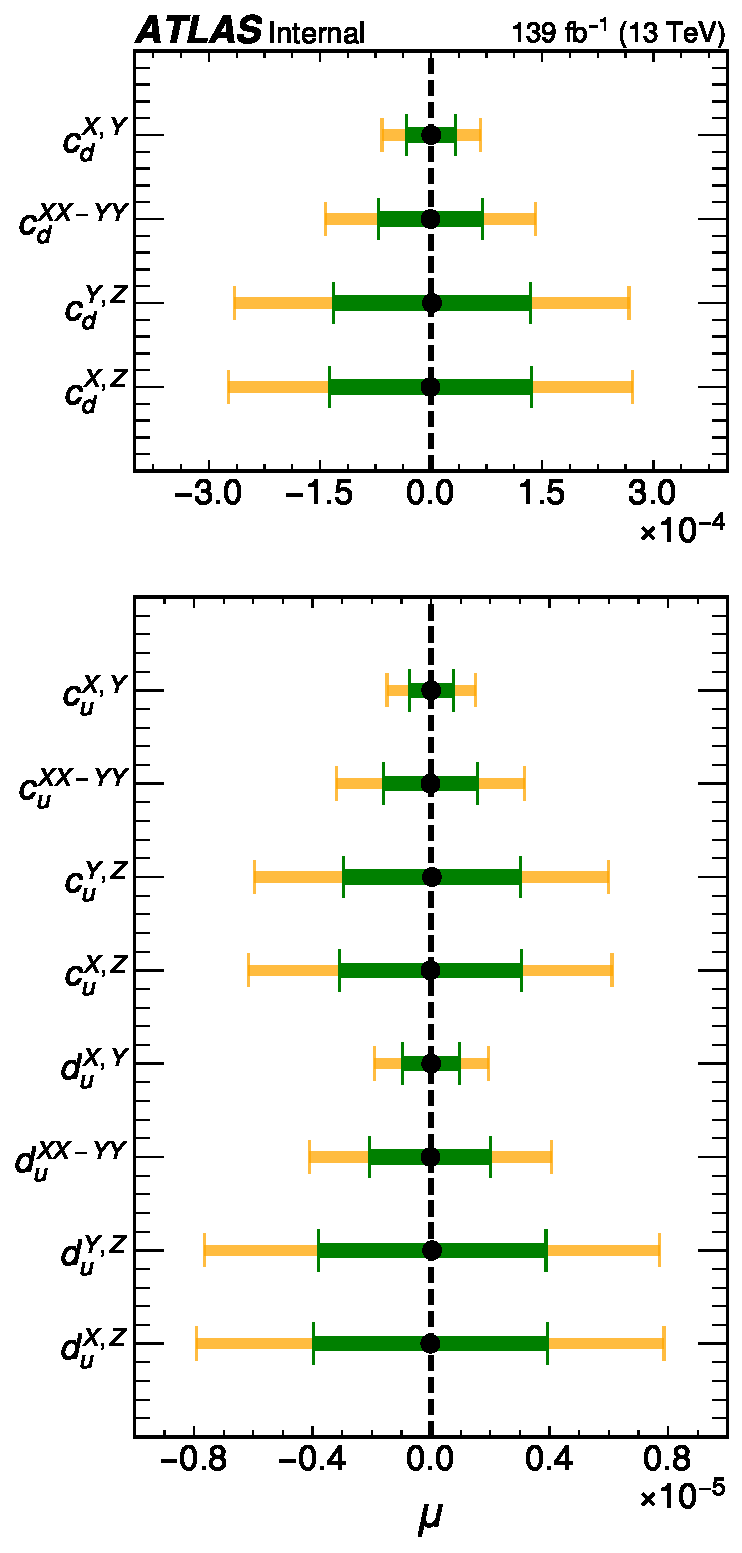
\includegraphics[width=0.45\textwidth]{figs/scrambling/SigFit_summary_AllSamples_SM}
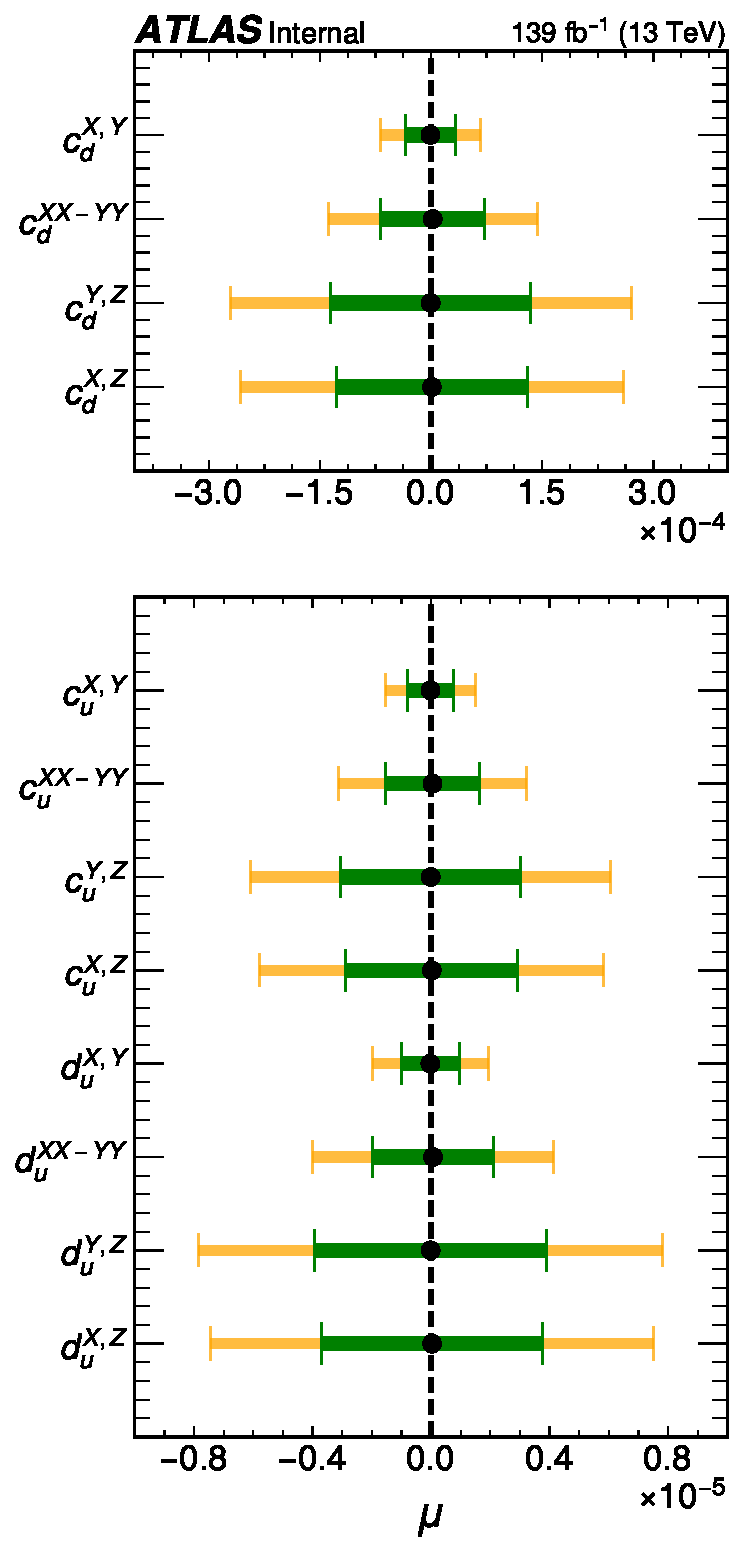
\includegraphics[width=0.45\textwidth]{figs/scrambling/SigFit_summary_AllSamples_SM_scrambled}
\caption{Fit results obtained from 1000 SM-like toy datasets. Results on SM-like toy 
datasets (left), which corresponds to full Run 2 luminosity, and scrambled SM-like 
toy datasets (right). SM-like toys are signal-free datsets ($\sigma_{LIV}/\sigma_{SM} = 0$).
 Y-axis corresponds to 12 exact signal shapes from SME. The X-axis is the signal strength.
  Yellow and green bends correspond to one and two signal uncertainty bands. }
\label{fig:SM_like_toy_fit_results12}
\end{figure}


%%%%%%%%%%%%%%%%%%%%%%%%%%%%%%%%%%%%%%%%%%%%%%%%%%%%%%
%%%%%%%%%%%%%%%%%%%%%%%%%%%%%%%%%%%%%%%%%%%%%%%%%%%%%%
%%%%%%%%%%%%%%%%%%%%%%%%%%%%%%%%%%%%%%%%%%%%%%%%%%%%%%
\subsection{Signal injected toys}

In this section, we present toy datasets in which signal injected
 at different signal amplitude for a singal shape $d_{u}^{X,Z}$. 
 The signal amplitude is $\sigma_{LIV}/\sigma_{SM}$. 
 In figure~\ref{fig:signal_injected_toy_p003_p0015}, one of the 1000 toys
  with signal amplitude 0.0009 (left plot) and 0.0022 (right plot)
   is compared to a fitted model, $d_{u}^{X,Z}$.

   In figure~\ref{fig:signal_injected_toy_p003_p0015_fit_results12}, we present average of 
   1000 fit results from signal injected toys. We can see that when
    $\sigma_{LIV}/\sigma_{SM}=0.009$ we already seeing a few sigma 
    deviation of the average value from zero (zero is SM expectation). And the deviation
     is even larger for larger signal. As we can see in both plots,
      there are three coefficients, $d_{u}^{X,Z}$, $c_{u}^{X,Z}$ and $c_{d}^{X,Z}$ show deviation.
      This is due to that these three signal shapes have very similar shape. Therefore, 
      when the $d_{u}^{X,Z}$ is injected, other two coefficients also show some deviation from zero.


\begin{figure}[hp]
\centering
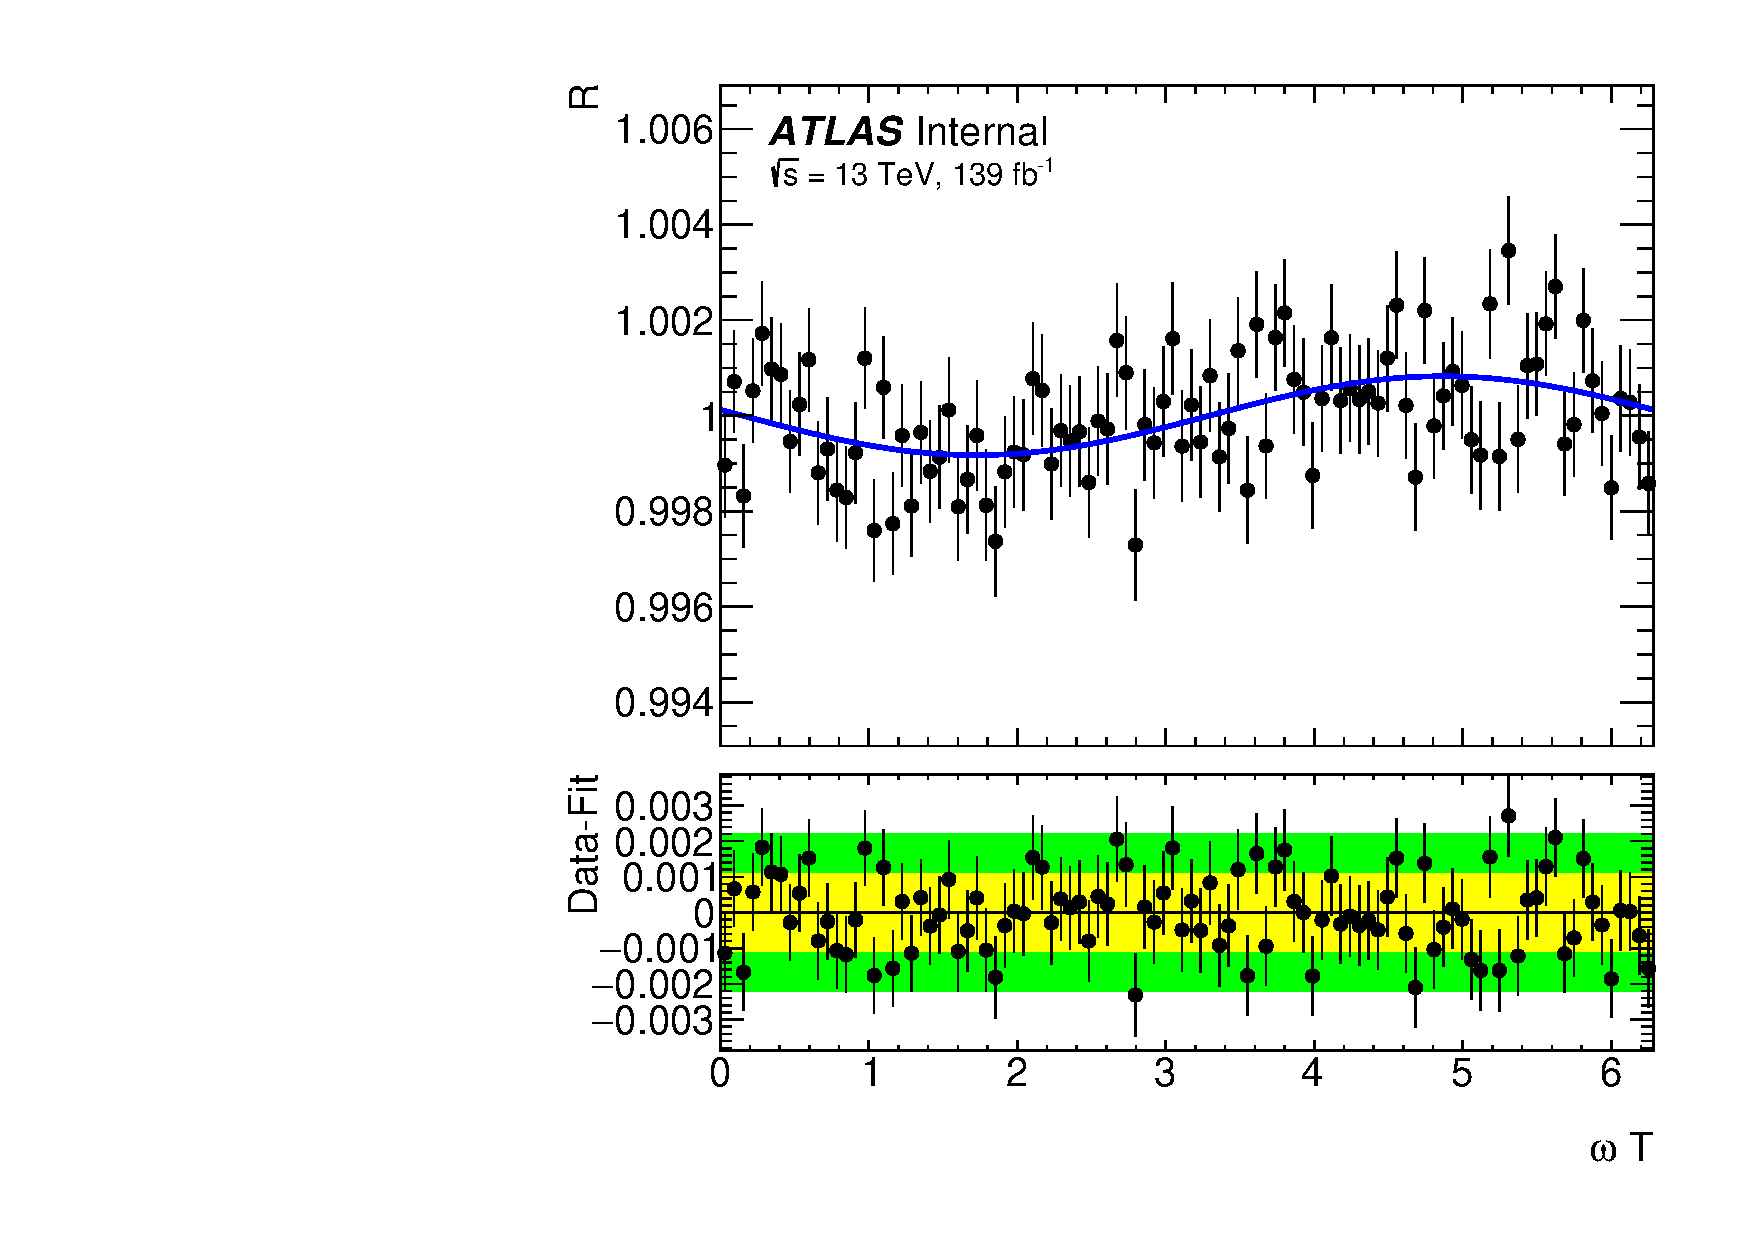
\includegraphics[width=0.45\textwidth]{figs/scrambling/fit_results_d[u,X,Z]_101_residual_12func_sigP0015}
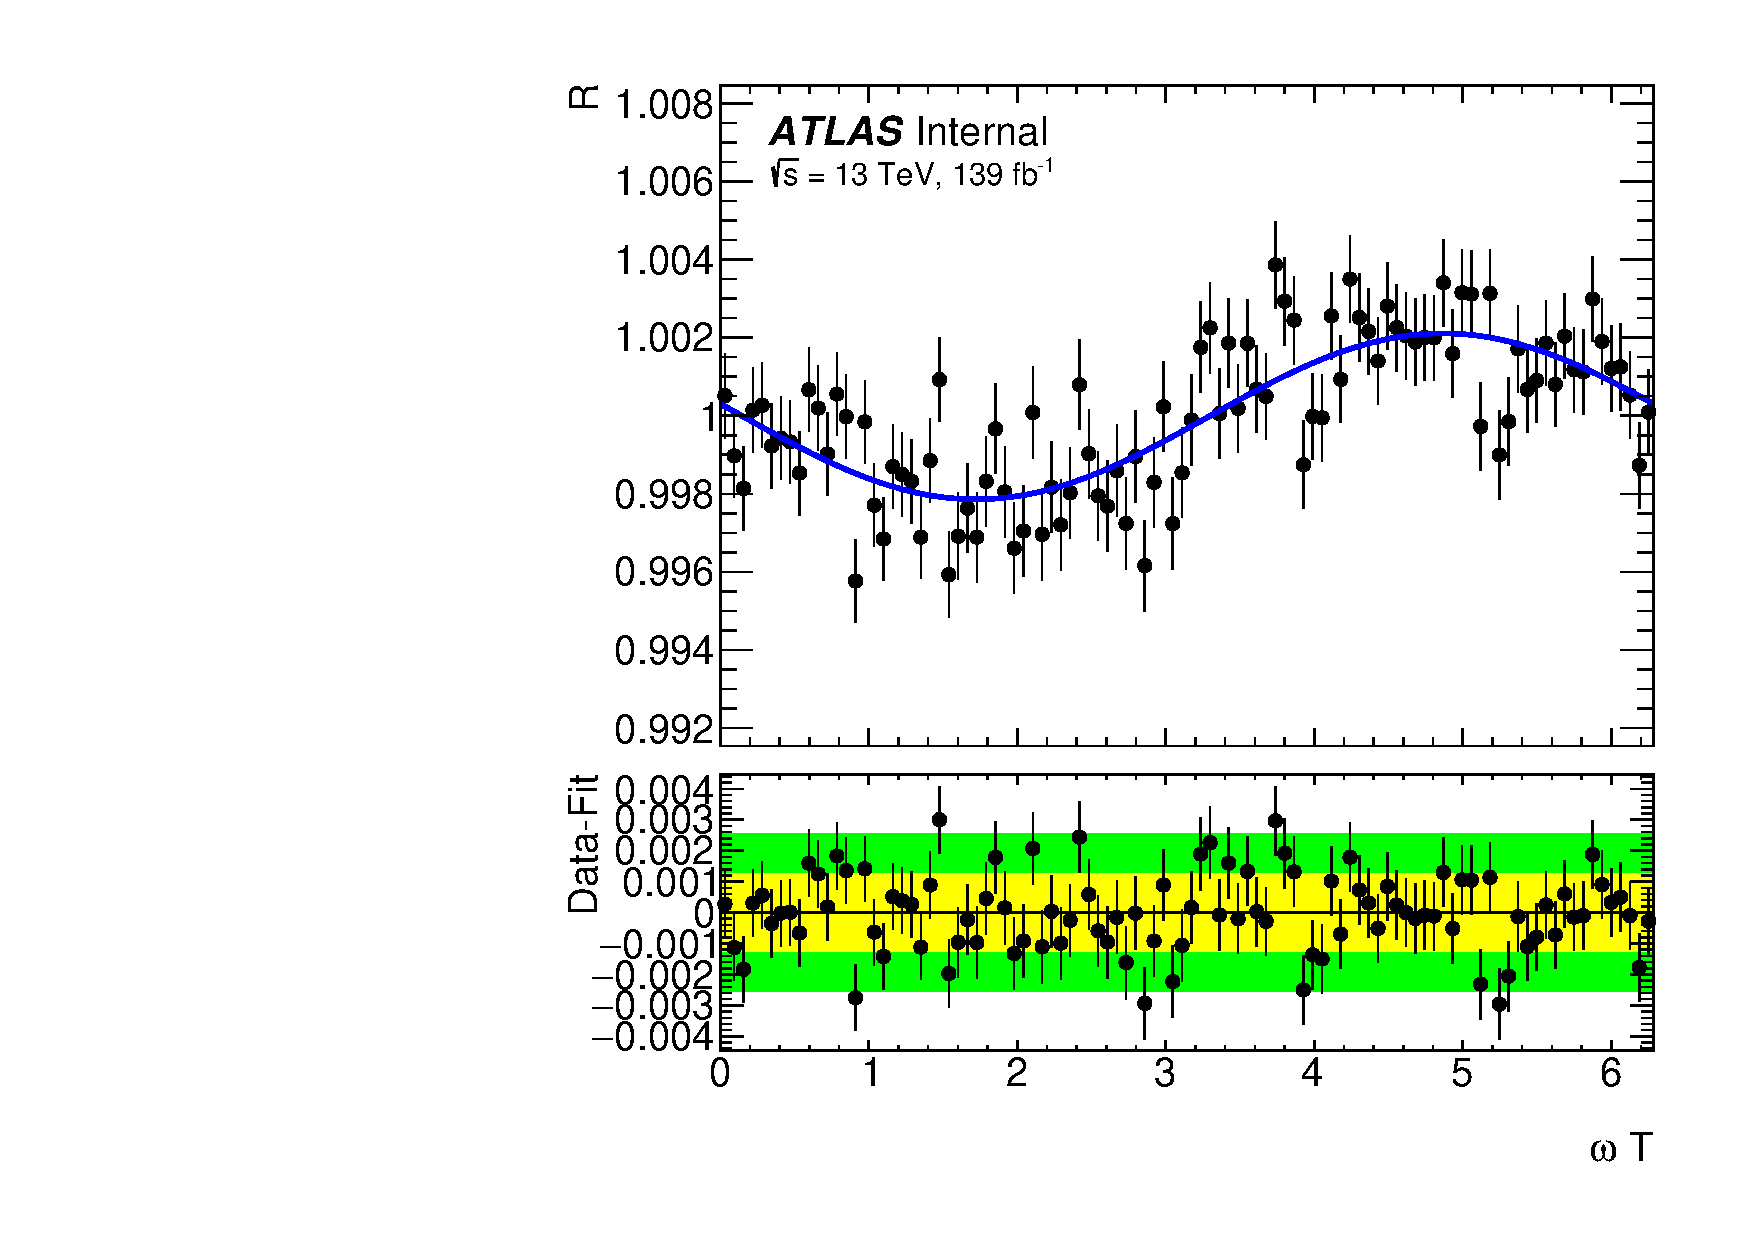
\includegraphics[width=0.45\textwidth]{figs/scrambling/fit_results_d[u,X,Z]_101_residual_12func_sigP003}
\caption{A signal injected toy dataset. The injected signal shape is $d_{u}^{X,Z}$ from SME. The njected 
signal fractions ($\sigma_{LIV}/\sigma_{SM}$)  are 0.0009 (left) and 0.0022 (right). The blue line is the
 signal ($d_{u}^{X,Z}$) after fit to the toy dataset. Bottom panel in each plot is the residual (data-fit).
  The X-axis is the sidereal phase, $\omega  T$.}
\label{fig:signal_injected_toy_p003_p0015}
\end{figure}




\begin{figure}[hp]
\centering
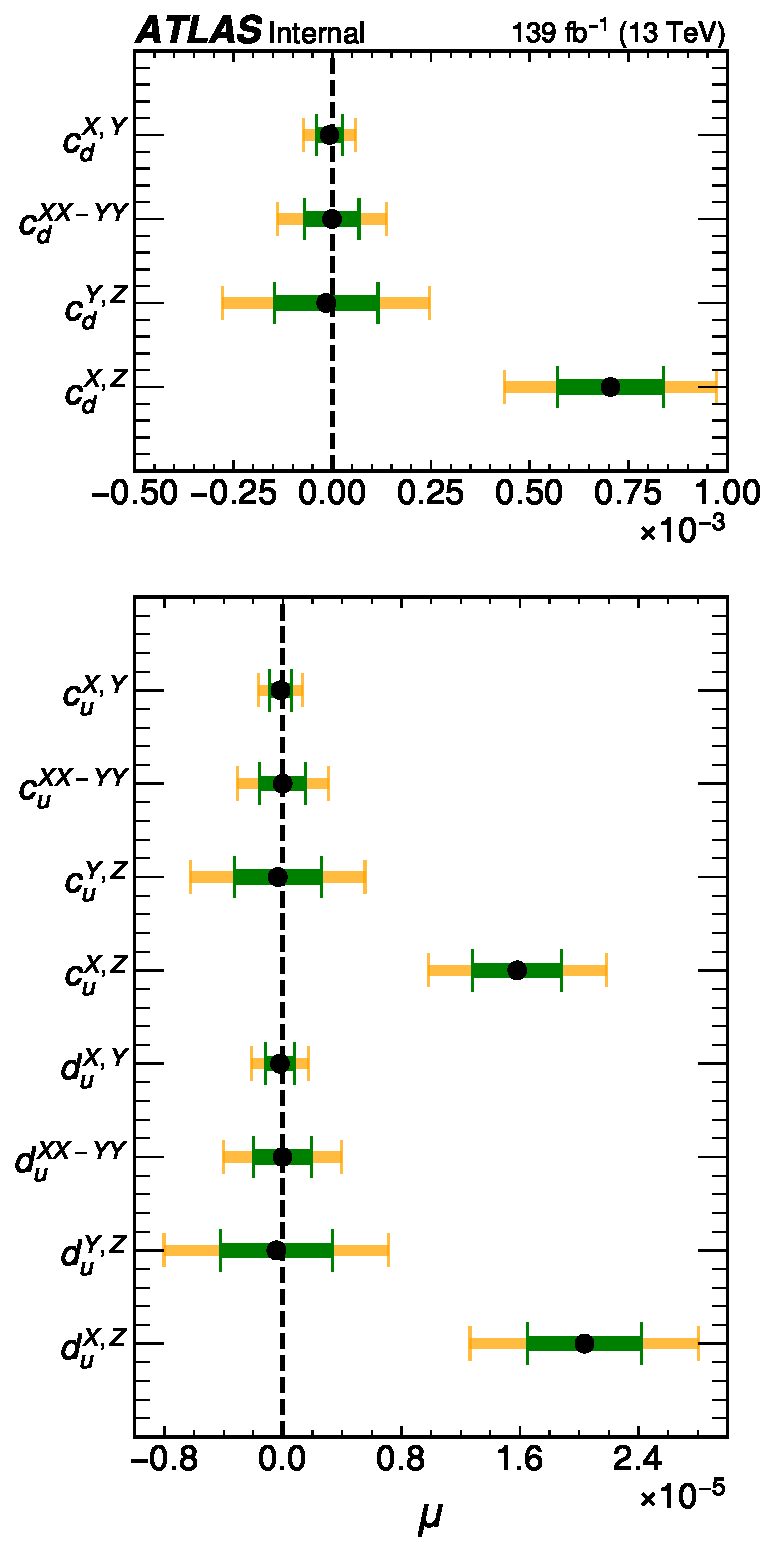
\includegraphics[width=0.45\textwidth]{figs/scrambling/SigFit_summary_AllSamples_sigP0015}
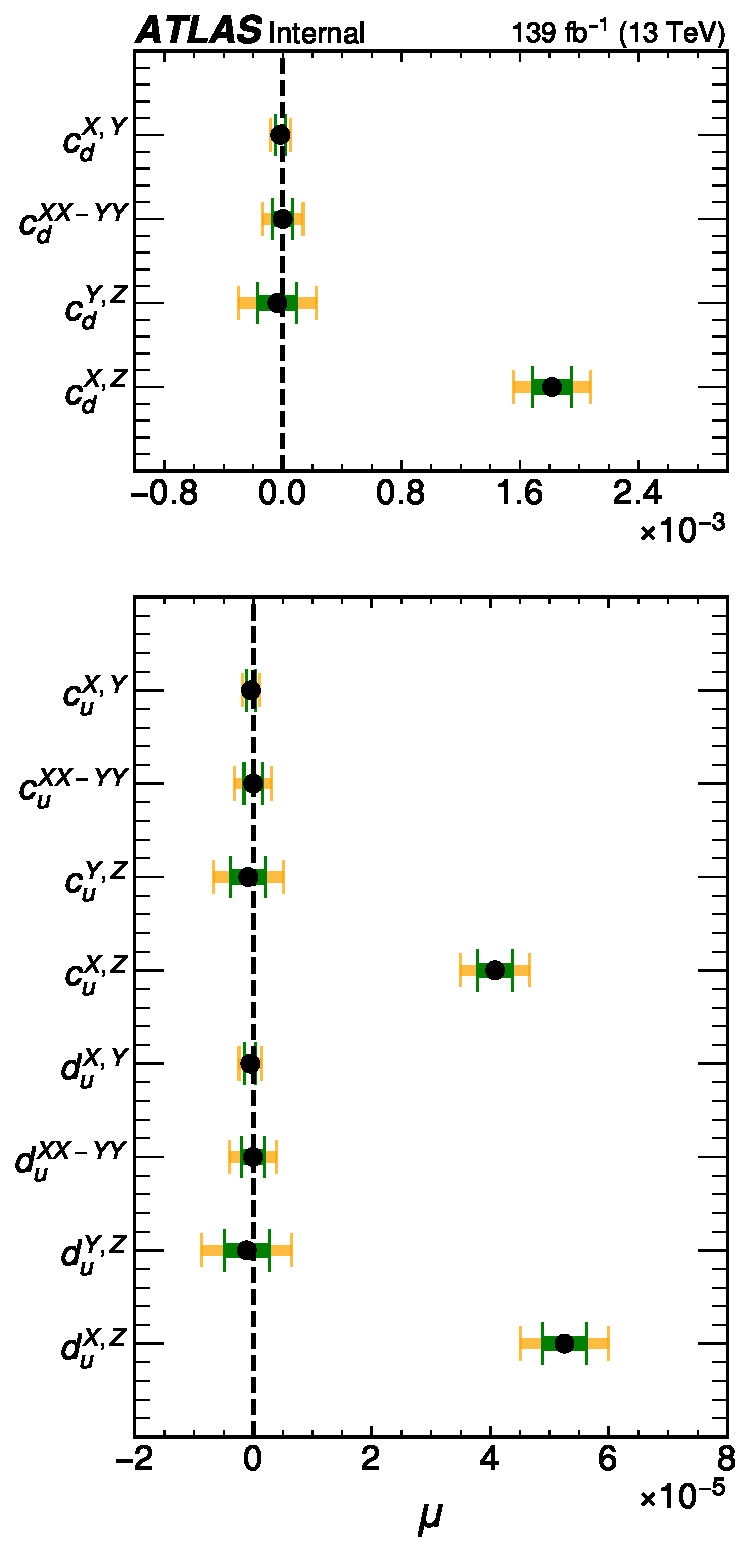
\includegraphics[width=0.44\textwidth]{figs/scrambling/SigFit_summary_AllSamples_sigP003}
\caption{Fit results from 1000 signal injected toys. The injected signal shape is $d_{u}^{X,Z}$ from SME.
 The njected signal fractions ($\sigma_{LIV}/\sigma_{SM}$)  are 0.0009 (left) and 0.0022 (right). 
 Y-axis corresponds to 12 exact signal shapes from SME. The X-axis is the signal strength.}
\label{fig:signal_injected_toy_p003_p0015_fit_results12}
\end{figure}



%%%%%%
%Scrambled signal injected toy.
%%%%%%
To proof the scrambling can perfectly wash away signals if they are in the real data,
 we applied scrambling to signal injected toys. 
 In figure~\ref{fig:signal_injected_toy_p003_beforeAfter_scramble} shows a signal injected 
 toy before (left) and after the scrambling (right). We can see from the left plot that signal 
 is strong, and the fitted singal strenth is $5.3E^{-5}\pm 3.8E^{-6}$. Still, 
the scrambling method washed away such a strong signal. The fitted signal strength is resuced 
to $-4.4E^{-7}\pm 3.8E^{-6}$ which is very good agreement with zero. 
Since toy datasets are distributed accourding to only statistical fluctuation we expect that 
the toy dataset after scrambling give similar results as SM like toys.
 


\begin{figure}[hp]
\centering
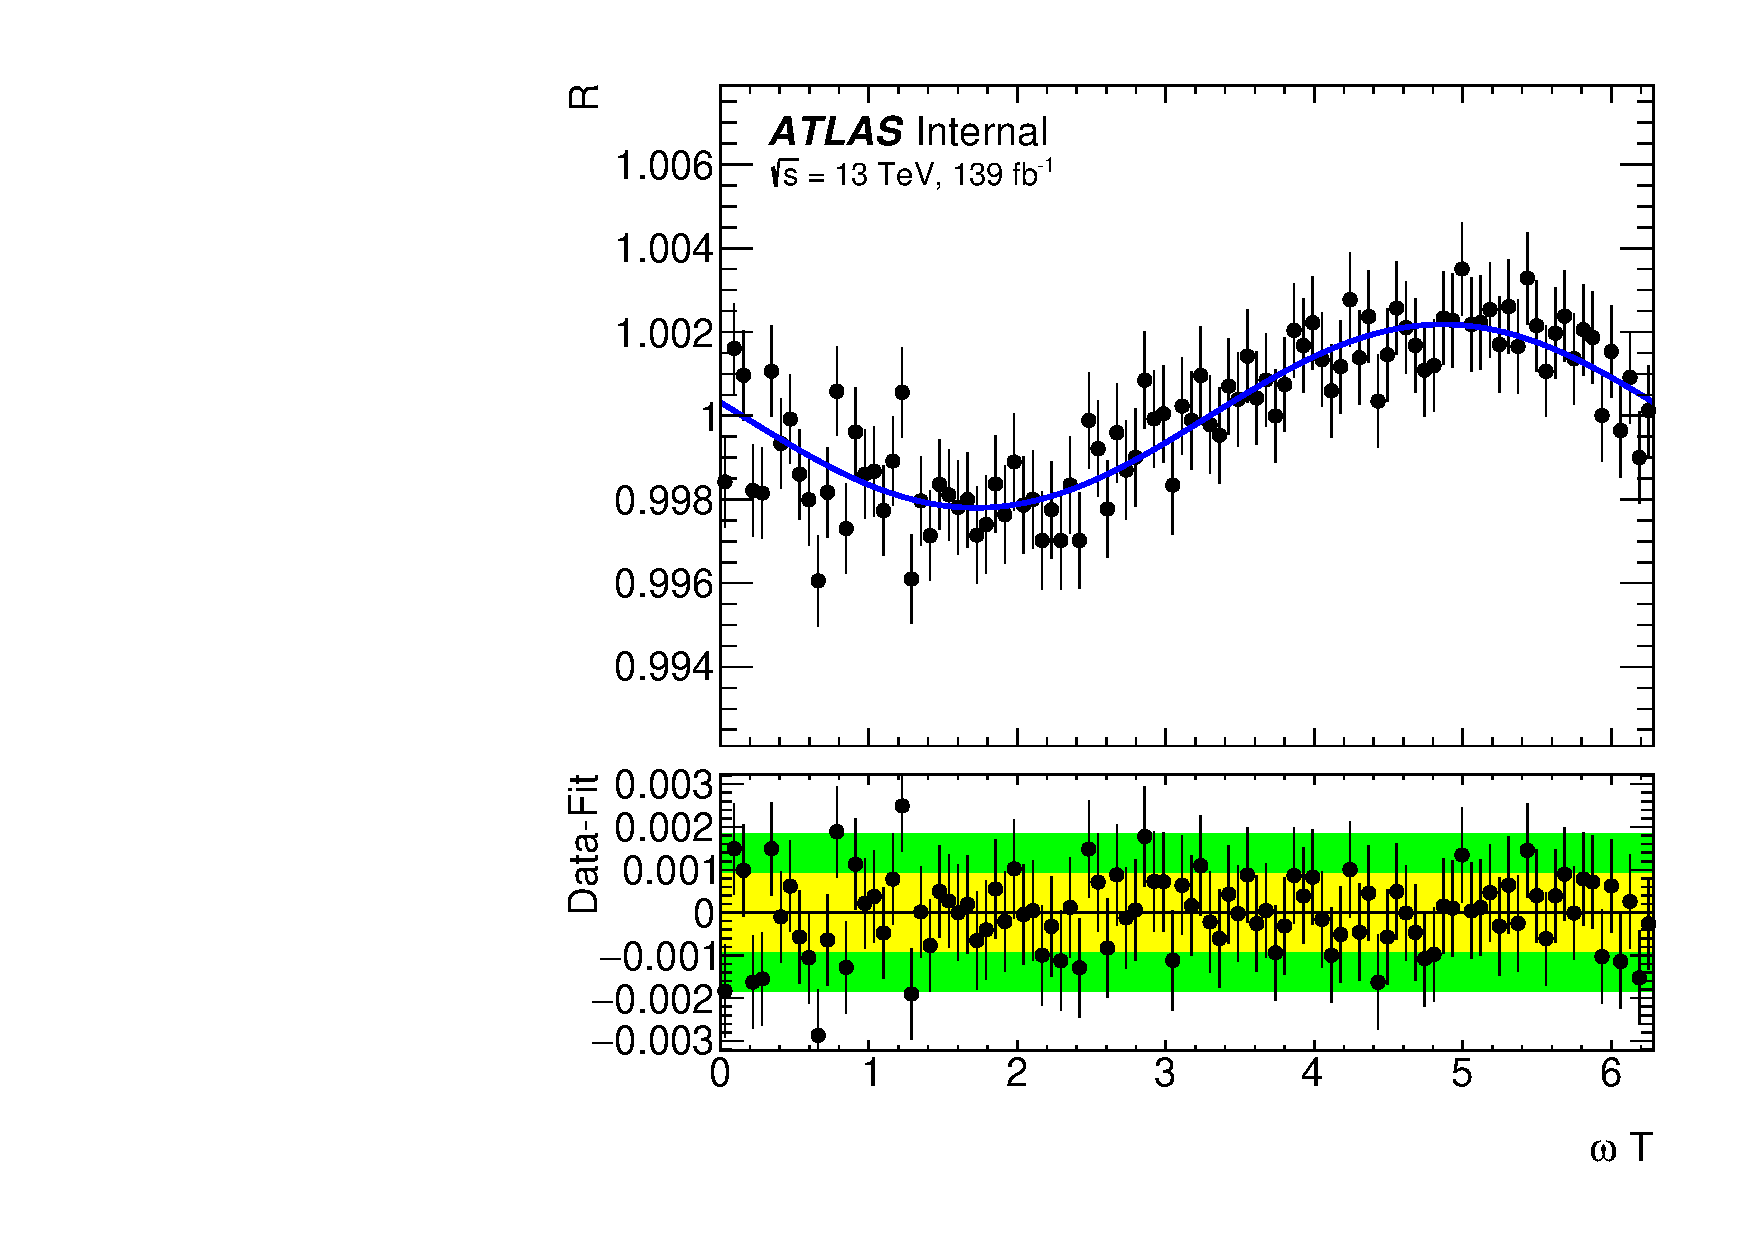
\includegraphics[width=0.45\textwidth]{figs/scrambling/fit_results_d[u,X,Z]_5170_residual_12func_sigP003}
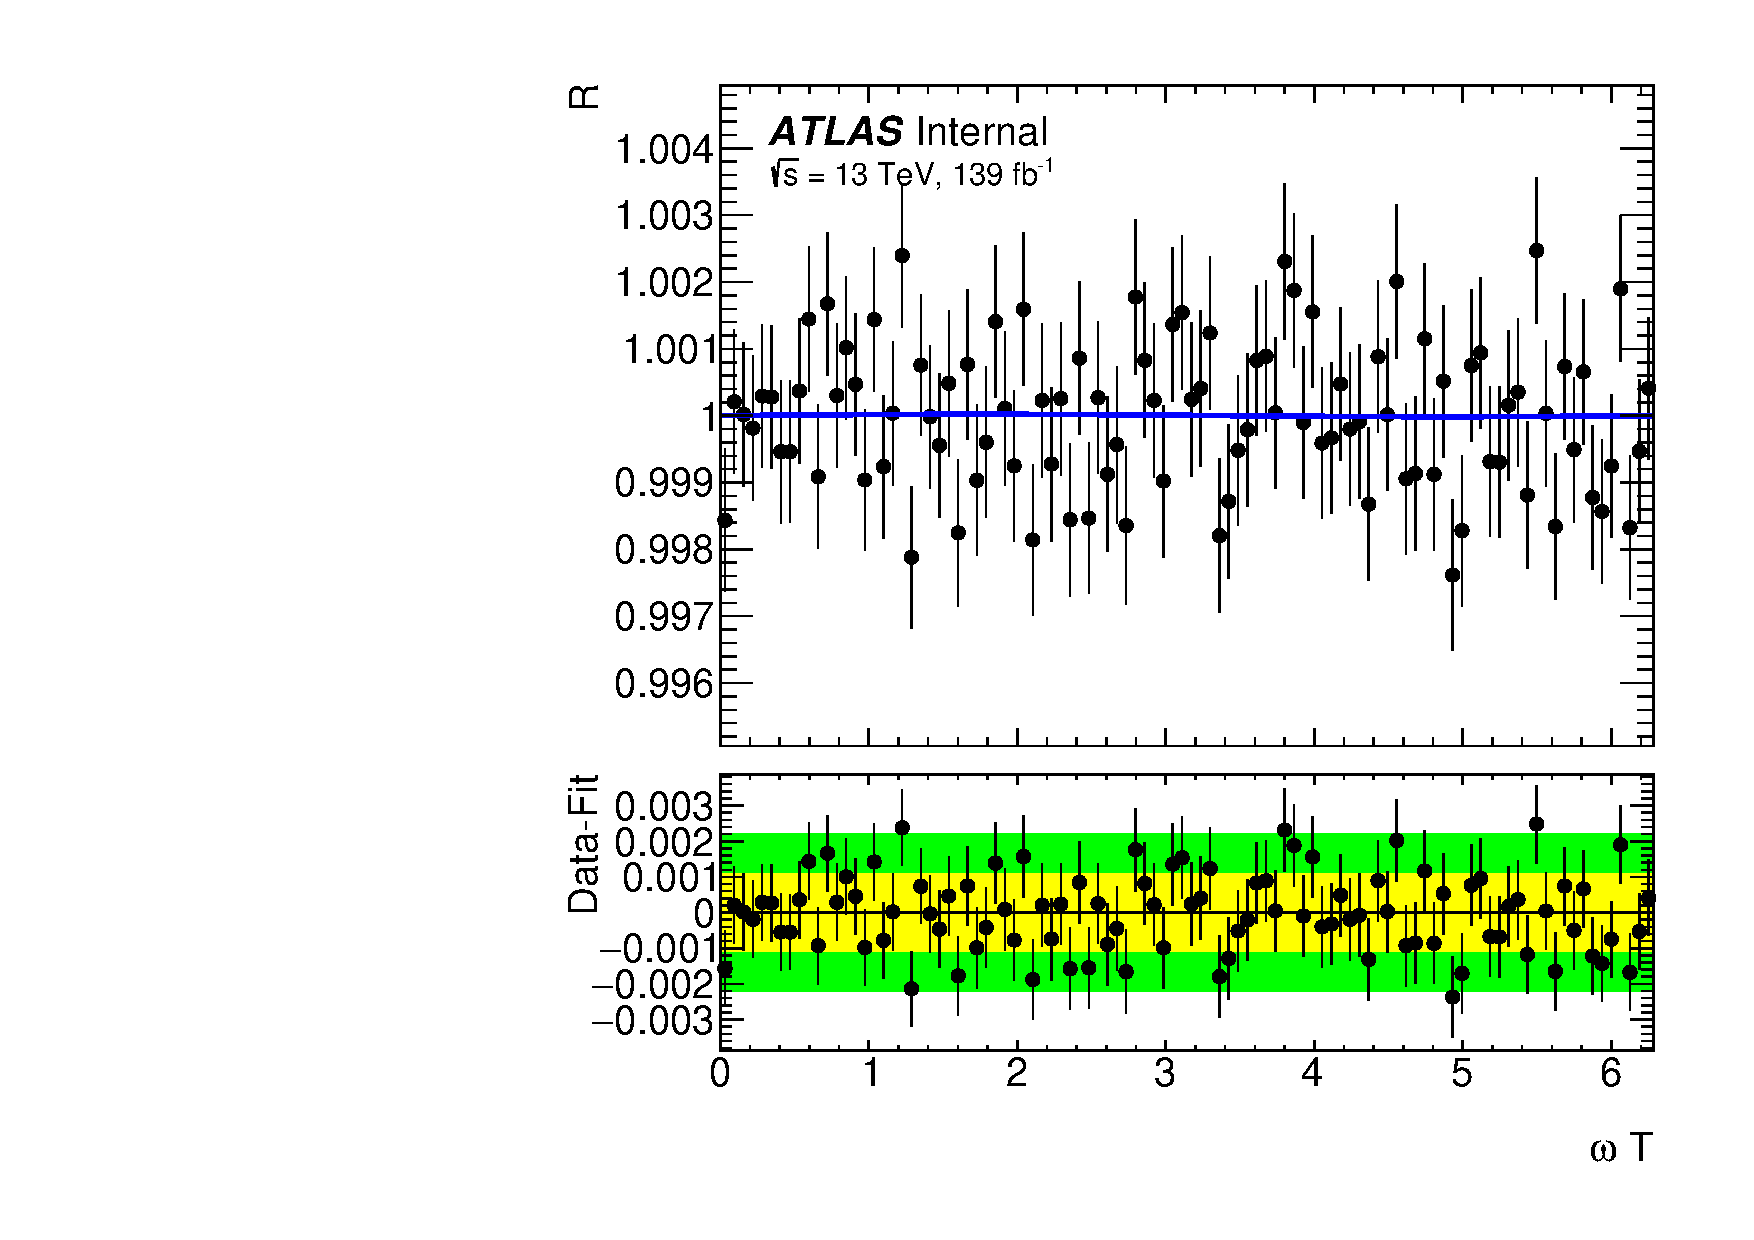
\includegraphics[width=0.45\textwidth]{figs/scrambling/fit_results_c[d,X,Z]_5170_residual_12func_sigP003_scrambled}
    \caption{Comparison of a signal injected toy dataset before and after a scramble. The injected signal shape 
    is $d_{u}^{X,Z}$ from SME. The injected signal fractions ($\sigma_{LIV}/\sigma_{SM}$)  is 0.0022. The original toy 
    dataset (left) and scrambled data (right). The blue line is the signal ($d_{u}^{X,Z}$) after fit to the toy dataset.
     The bottom panel in each plot is the residual (data - fit). The X-axis is the sidereal phase, $\omega T$.
The Fitted signal strength is $5.3E^{-5}\pm 3.8E^{-6}$ (left), and $-4.4E^{-7}\pm 3.8E^{-6}$ (right) after scrambling. 
}
\label{fig:signal_injected_toy_p003_beforeAfter_scramble}
\end{figure}
